\begin{figure}[H]
\centering
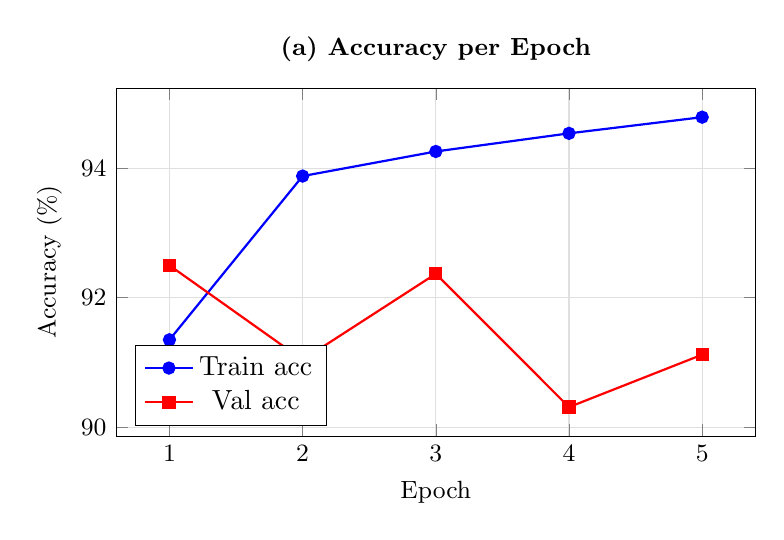
\begin{tikzpicture}
\begin{axis}[width=0.8\linewidth, height=6cm,
    title={\textbf{(a) Accuracy per Epoch}}, title style={font=\small\bfseries},
    xlabel={Epoch}, ylabel={Accuracy (\%)}, legend pos=south west,
    xtick={1,2,3,4,5}, grid=both, grid style={gray!25},
    tick label style={font=\small}, label style={font=\small}]
\addplot[blue, mark=*, thick] coordinates {(1,91.35) (2,93.88) (3,94.26) (4,94.54) (5,94.78999999999999)};
\addlegendentry{Train acc}
\addplot[red, mark=square*, thick] coordinates {(1,92.5) (2,91.03999999999999) (3,92.36999999999999) (4,90.31) (5,91.12)};
\addlegendentry{Val acc}
\end{axis}\end{tikzpicture}

\vspace{0.6em}
\begin{tikzpicture}
\begin{axis}[width=0.8\linewidth, height=6cm,
    title={\textbf{(b) Loss and Validation Macro-F1}}, title style={font=\small\bfseries},
    xlabel={Epoch}, ylabel={Value}, legend pos=east,
    xtick={1,2,3,4,5}, grid=both, grid style={gray!25},
    tick label style={font=\small}, label style={font=\small}]
\addplot[blue, mark=*, thick] coordinates {(1,0.217) (2,0.158) (3,0.1473) (4,0.1386) (5,0.1327)};
\addlegendentry{Train loss}
\addplot[red, mark=square*, thick] coordinates {(1,0.1679) (2,0.1954) (3,0.1856) (4,0.2086) (5,0.1957)};
\addlegendentry{Val loss}
\addplot[green!55!black, mark=triangle*, thick] coordinates {(1,0.8894) (2,0.8796) (3,0.8874) (4,0.876) (5,0.8811)};
\addlegendentry{Val Macro-F1}
\end{axis}\end{tikzpicture}
\caption[Stage 3 training curves]{Stage~3 fusion training dynamics over 5 epochs,
measured on the auxiliary question-type routing head. The best validation
accuracy (92.50\%) is reached at epoch~1; later epochs slightly overfit, so the
epoch-1 checkpoint is retained.}
\label{fig:stage3_curves}
\end{figure}
